% !TeX document-id = {3ffda977-020f-403a-a748-6559a1e64ed1}
% !TeX TXS-program:compile = txs:///pdflatex/[--shell-escape]
% % !TEX TS-program = xelatex
% !TEX encoding = UTF-8 Unicode


% Spring 2020 - Summer 2020 - Fall 2020 - SPring 2021
% Tristan Hill, May 07, 2020 - June 12, 2020 - July 08, 2020 - Novemeber 02, 2020 - March 28, 2021
% Module Name: - Electrical Signals
% Topic 1 - Introduction to Electrical Signals

\documentclass[fleqn]{beamer} % for presentation (has nav buttons at bottom)

\usepackage{/home/thill/Documents/lectures/measurements_lectures/measurements_lectures}


\author{ME3023 - Measurements in Mechanical Systems} % original formatting from Mike Renfro, September 21, 2004

\newcommand{\MNUM}{9\hspace{2mm}} % Module number - The module number should be phased out...
\newcommand{\TNUM}{1\hspace{2mm}} % Topic number - Topic numbers are going to stay
\newcommand{\moduletitle}{Electrical Signals}
\newcommand{\topictitle}{Classification of Signals  } 

\newcommand{\sectiontitleI}{Introduction to Signal Concepts}
\newcommand{\sectiontitleII}{Analog, Discrete, or Digital}
\newcommand{\sectiontitleIII}{Static or Dynamic}
\newcommand{\sectiontitleIV}{Deterministic or Non-Deterministic}

\newcommand{\btVFill}{\vskip0pt plus 1filll}


% custom box
\newsavebox{\mybox}

\title{Lecture Module - \moduletitle}

\date{Mechanical Engineering\vspc Tennessee Technological University}

\begin{document}

\lstset{language=MATLAB,basicstyle=\ttfamily\small,showstringspaces=false}

\frame{\titlepage \center\begin{framed}\Large \textbf{Topic \TNUM - \topictitle}\end{framed} \vspace{5mm}}

% Section 0: Outline
\frame{
\large \textbf{Topic \TNUM - \topictitle} \vspace{3mm}\\

\begin{itemize}

	\item \sectiontitleI    \vspc % Section I
	\item \sectiontitleII 	\vspc % Section II
	\item \sectiontitleIII 	\vspc %Section III
	\item \sectiontitleIV 	\vspc %Section IV
%	\item \sectiontitleV 	\vspc %Section IV

\end{itemize}

}

% Section I:
\section{\sectiontitleI}

	% Section I - Frame I:
	\begin{frame}[label=sectionI] \small
		\frametitle{\sectiontitleI}
		
		{\RD Signal}, {\GR Amplitude}, and {\BL Frequency}\vspace{2mm}\\
		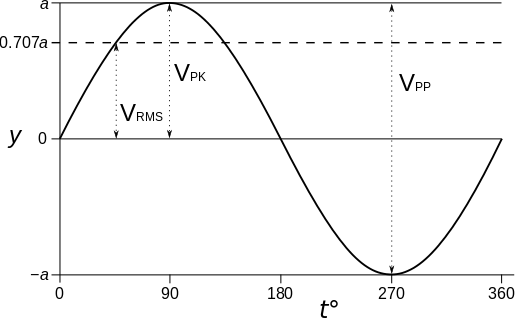
\includegraphics[scale=.25]{amplitude_frequency.png} 
		%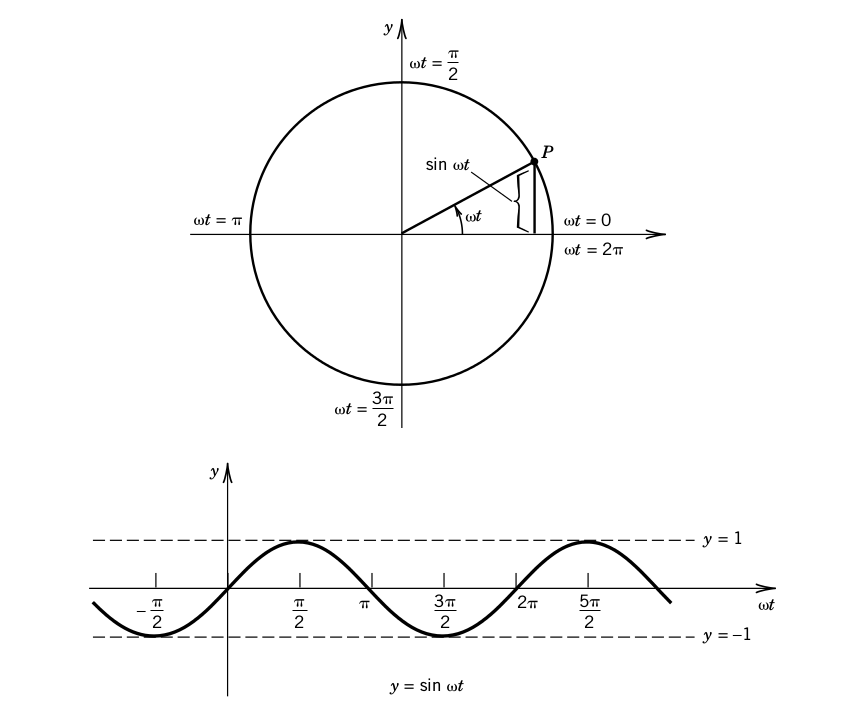
\includegraphics[scale=.25]{unit_circle.png}
		
		{\it The shape and form of a signal are often referred to as its waveform.
		The waveform contains information about the magnitude and amplitude, which indicate the size of
		the input quantity, and the frequency, which indicates the way the signal changes in time. }\vspace{5mm}\\
		
		\btVFill
		\tiny{Text: Theory and Design for Mechanical Measurements}
	\end{frame}

	% Section I - Frame II
	\begin{frame}[label=sectionI] \small
		\frametitle{\sectiontitleI}    				
		\bigskip
		
		{\it A {\PR signal} is the physical information about a measured variable being transmitted
		between a process and the measurement system, between the stages of a measurement system, or as
		the output from a measurement system. } \\
	
		
		\btVFill
		\tiny{Text: Theory and Design for Mechanical Measurements}	
	\end{frame}


\section{\sectiontitleII}	
	% Section II - Frame I
	\begin{frame}[label=sectionII] \small
		\frametitle{\sectiontitleII}
		

	    \begin{itemize}
			\item \textbf{Analog Signal- magnitude is continuous in time }  \vspace{3mm} \\
			\item \textbf{Discrete Time Signal- magnitude at points in time}  \vspace{3mm} \\
			\textbf{ \hspace*{15mm} - sampling at repeated time intervals}  \vspace{3mm} \\
			\item \textbf{Digital Signal- exists in discrete points in time}  \vspace{3mm} \\
			\textbf{ \hspace*{15mm} - magnitude is also discrete}  \vspace{3mm} \\
		\end{itemize}
		
		
	\end{frame}

	% Section II - Frame II
	\begin{frame} \small
		\frametitle{\sectiontitleII}
		\bigskip    
		
		{\it {\RD Analog} describes a signal that is
		continuous in time. Because physical variables tend to be continuous, an analog signal provides a
		ready representation of their time-dependent behavior. }

		\vspace{30mm}
		Examples: voltage in a circuit
%	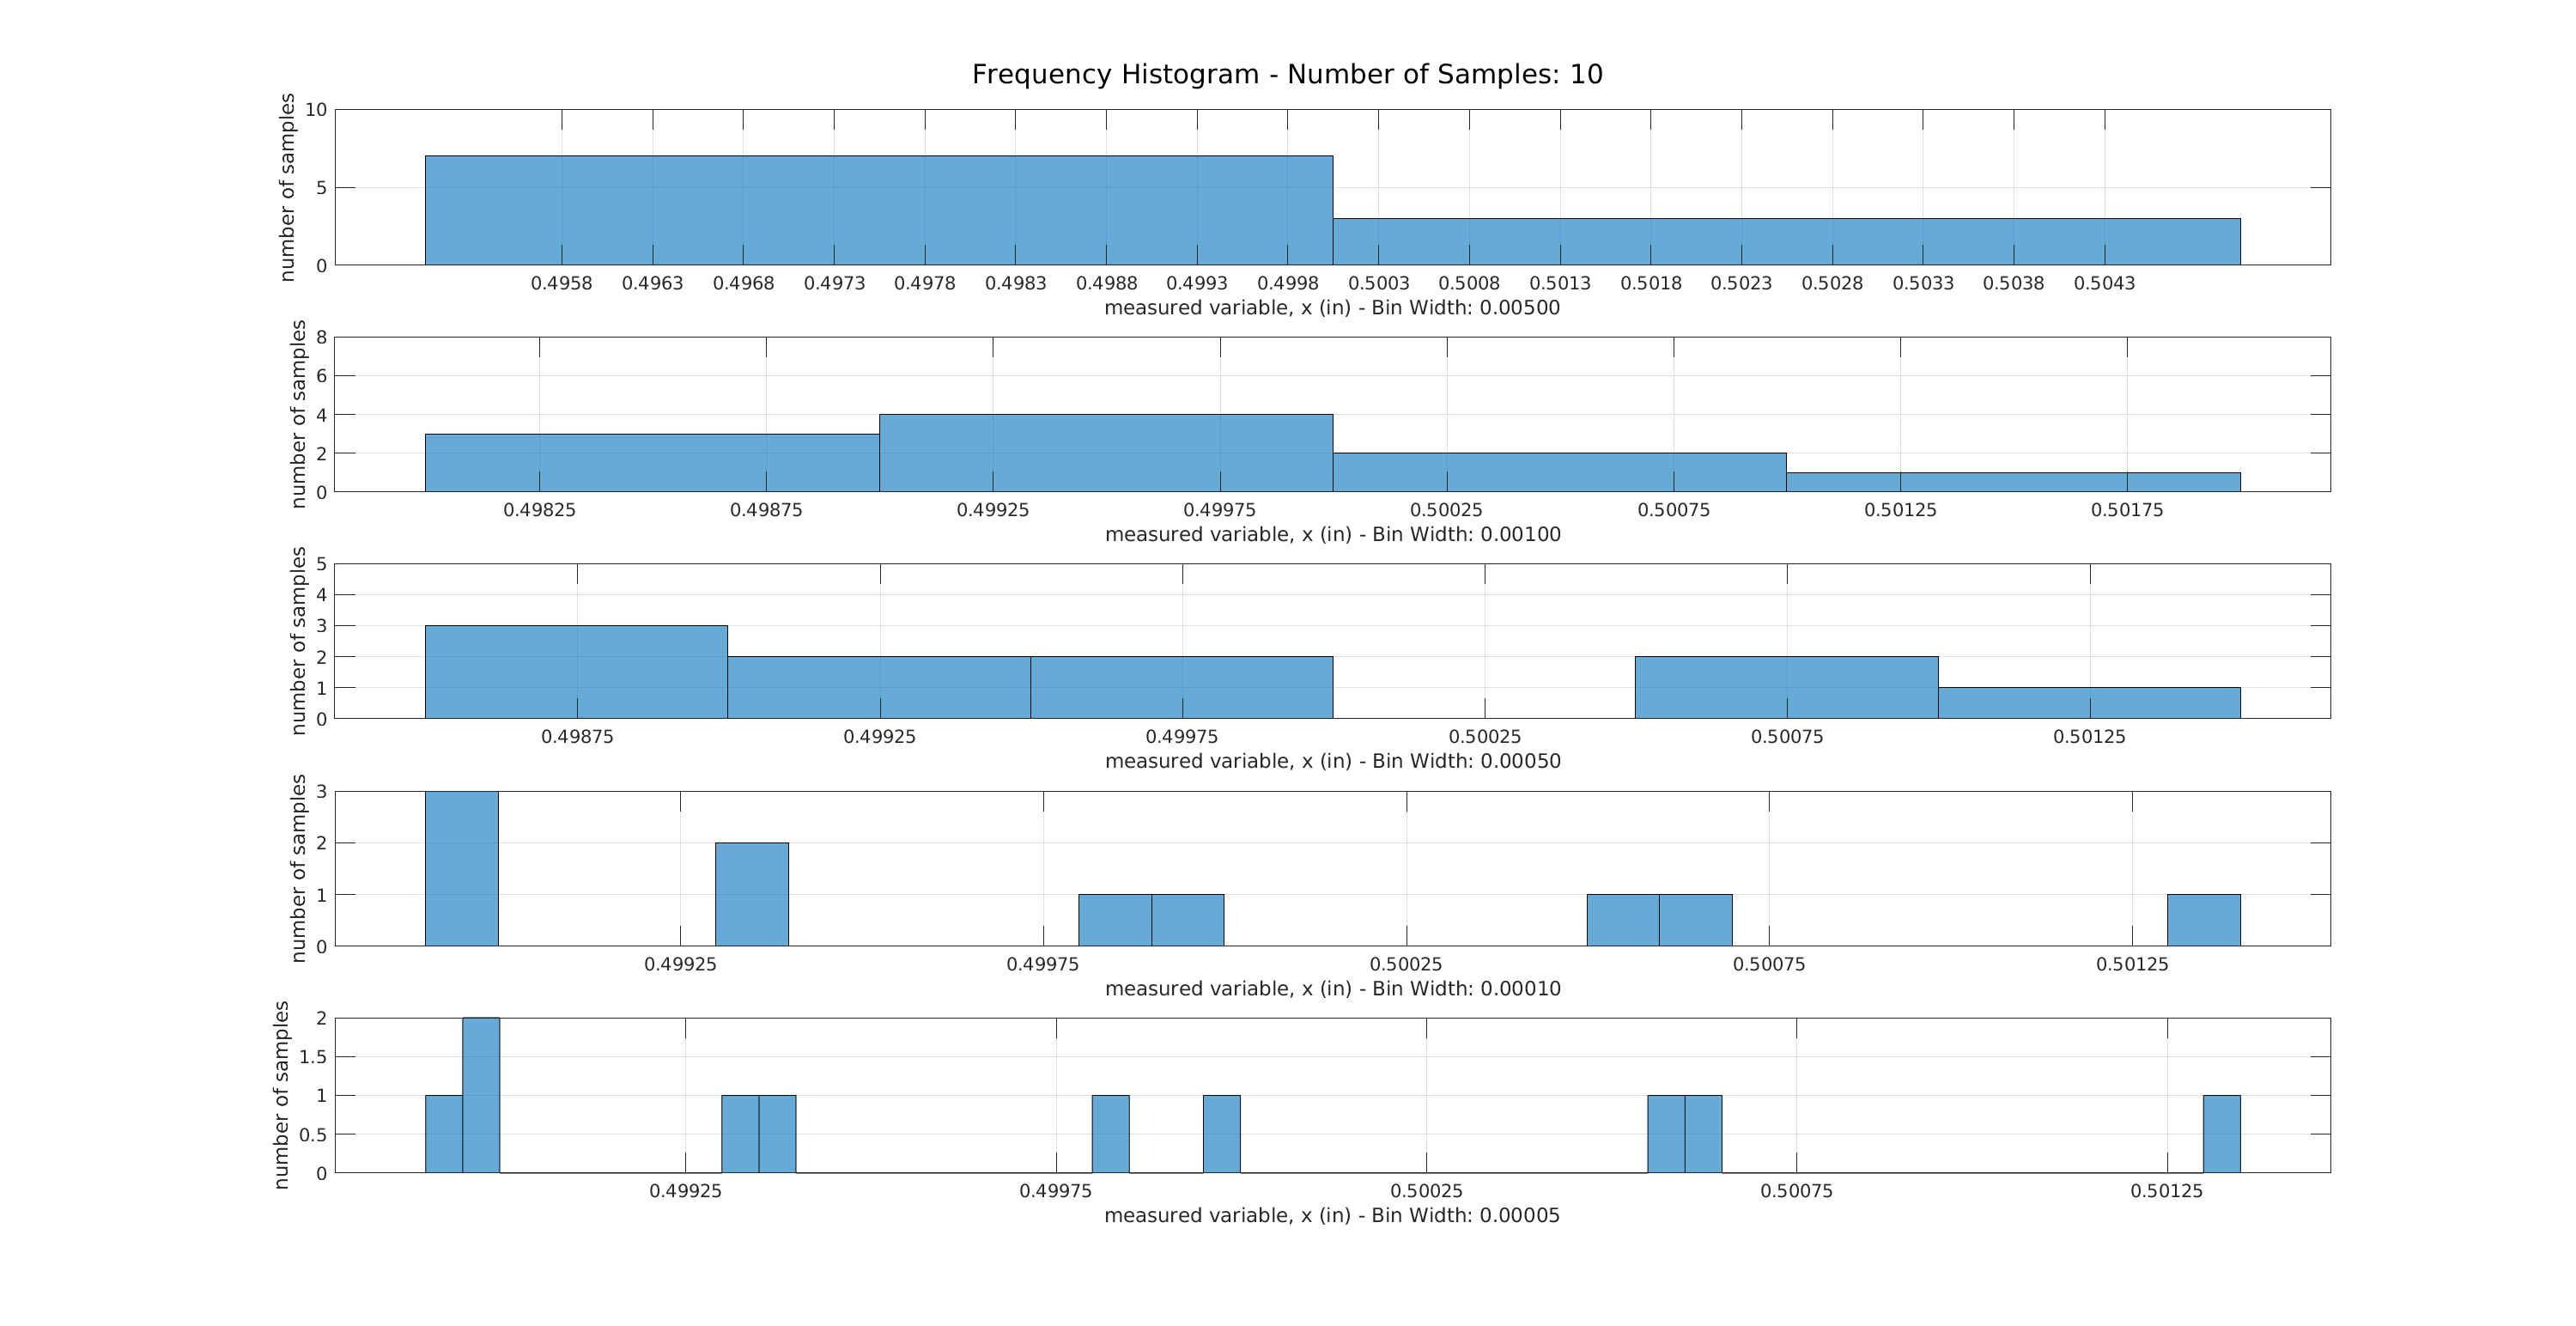
\includegraphics[scale=.25]{topic2_histogram_fig1}
		\btVFill
		\tiny{Text: Theory and Design for Mechanical Measurements}	
	\end{frame}
	
	% Section II - Frame III
	\begin{frame} \small
		\frametitle{\sectiontitleII}    
		\bigskip  
			
		{\it ...a {\GR discrete time} signal, for which information about the
		magnitude of the signal is available only at discrete points in time. A discrete time signal usually
		results from the sampling of a continuous variable at repeated finite time intervals. }

%	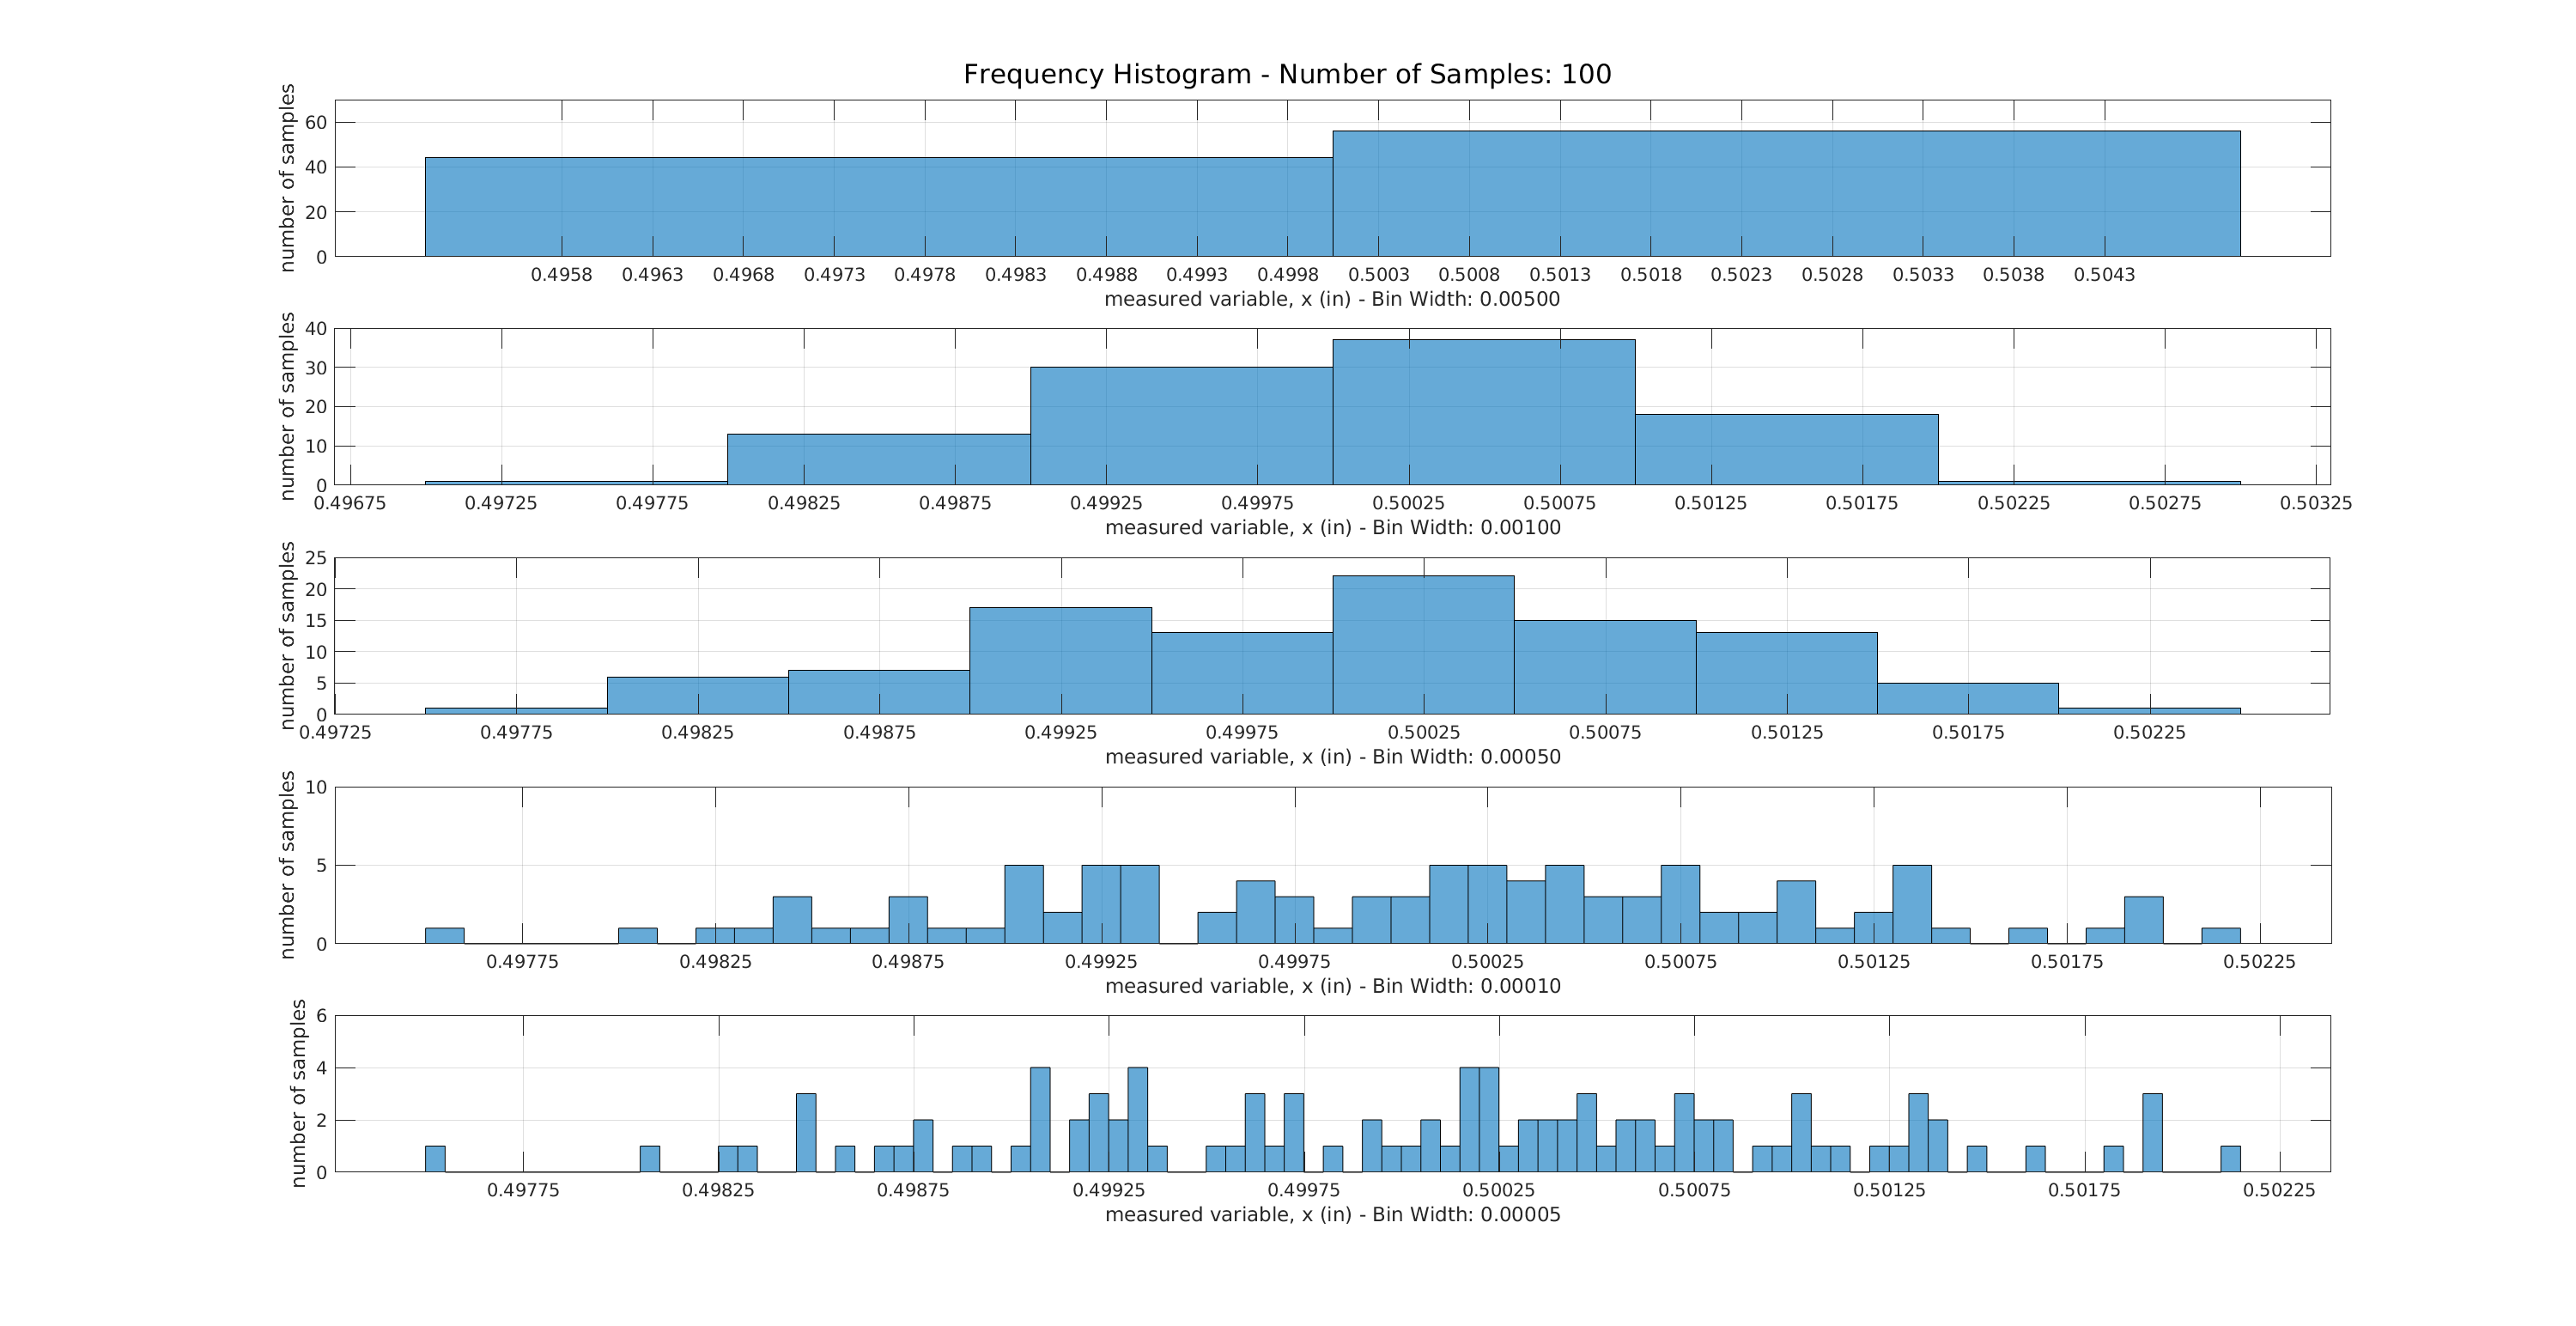
\includegraphics[scale=.25]{topic2_histogram_fig2}
		\vspace{30mm}
		Examples:
		\btVFill
		\tiny{Text: Theory and Design for Mechanical Measurements}	
	\end{frame}
	
	% Section II - Frame IV
	\begin{frame} \small
		\frametitle{\sectiontitleII}    
		\bigskip 
			{\it A {\BL digital} signal has two important characteristics. First, a digital signal
			exists at discrete values in time, like a discrete time signal. Second, the magnitude of a digital signal
			is discrete, determined by a process known as {\PR quantization} at each discrete point in time. }

%	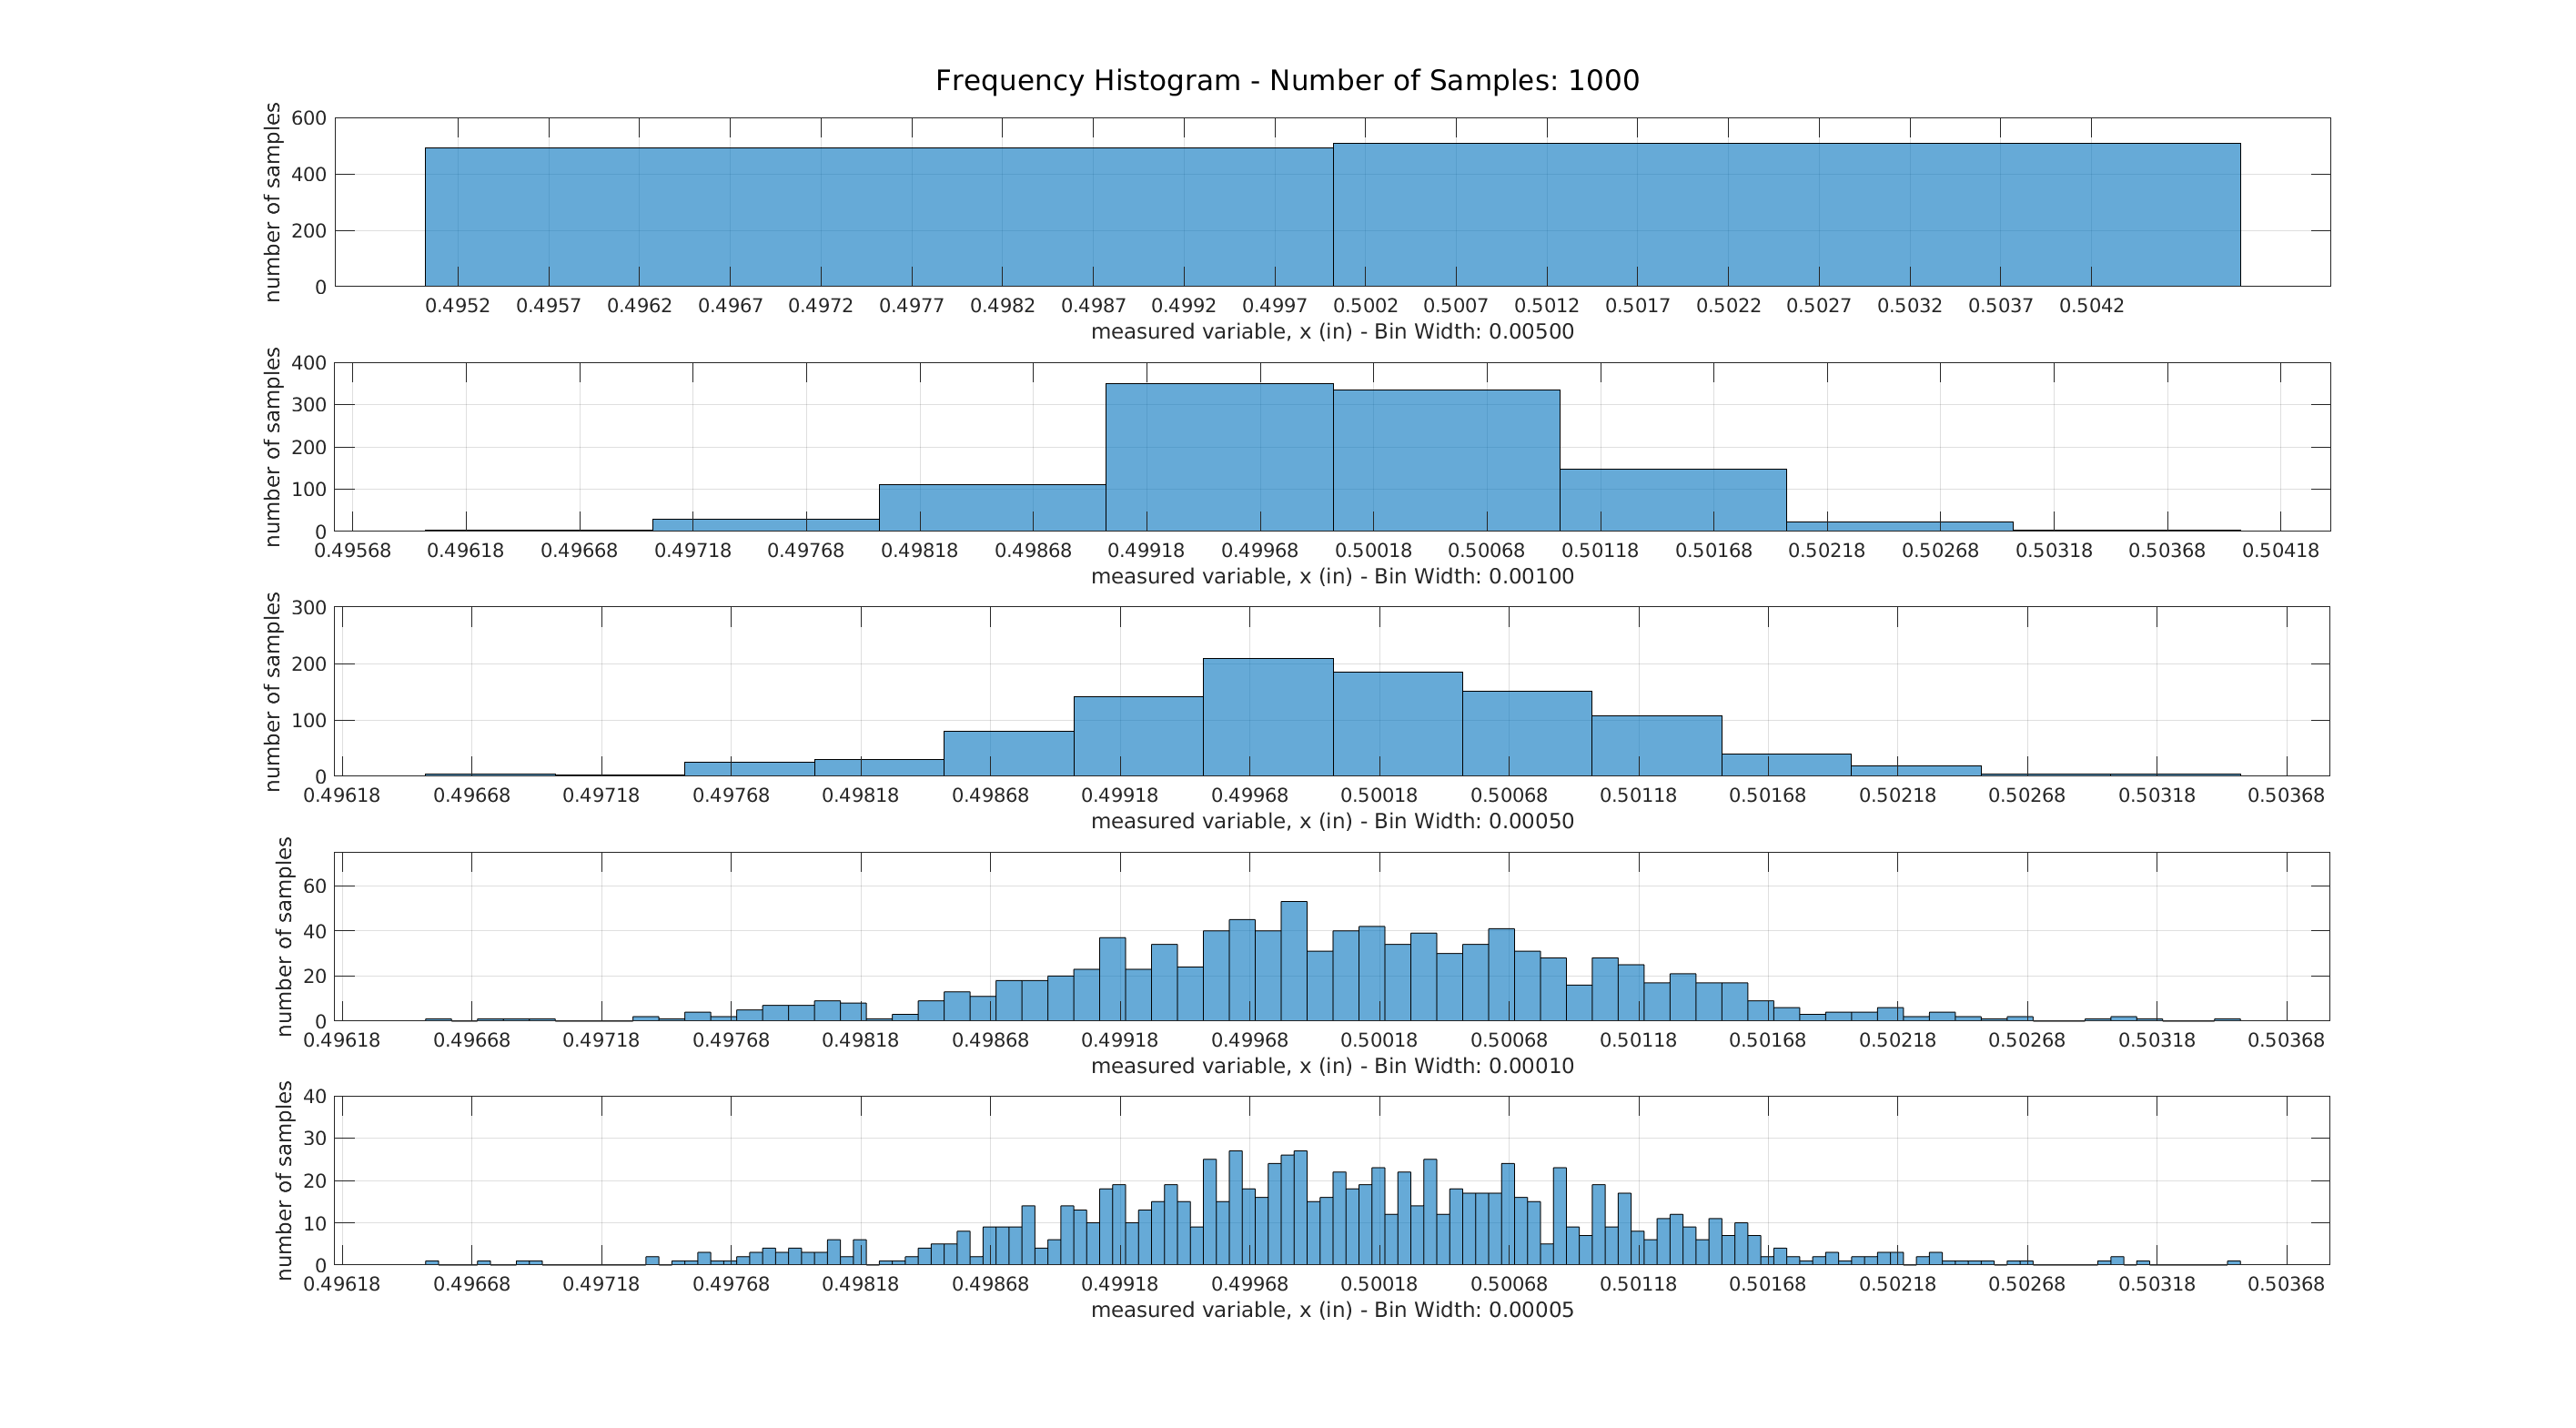
\includegraphics[scale=.25]{topic2_histogram_fig3}
		\vspace{30mm}
		Examples:
		\btVFill
		\tiny{Text: Theory and Design for Mechanical Measurements}	
	\end{frame}
	
\section{\sectiontitleIII}	
% Section III - Frame I
\begin{frame}[label=sectionIII] \small
\frametitle{\sectiontitleIII}
\bigskip

Signals may be characterized as either static or
dynamic. A static signal does not vary with time.

A dynamic signal is defined as a time-dependent signal. In general, dynamic signal waveforms,
y(t), may be classified as shown in Table 2.1.
	
\btVFill
\tiny{Text: Theory and Design for Mechanical Measurements}		
\end{frame}

\section{\sectiontitleIV}	
% Section IV - Frame I
\begin{frame}[label=sectionIV] \small
\frametitle{\sectiontitleIV}
\bigskip

A deterministic signal varies in time in a predictable
manner, such as a sine wave, a step function, or a ramp function, as shown in Figure 2.5. A signal is
steady periodic if the variation of the magnitude of the signal repeats at regular intervals in time.

Also described in Figure 2.5 is a nondeterministic signal that has no discernible pattern of
repetition. A nondeterministic signal cannot be prescribed before it occurs, although certain char-
acteristics of the signal may be known in advance.

\btVFill
\tiny{Text: Theory and Design for Mechanical Measurements}	
\end{frame}

% Section IV - Frame II
\begin{frame}[label=sectionIV] \small
\frametitle{\sectiontitleIV}
\bigskip

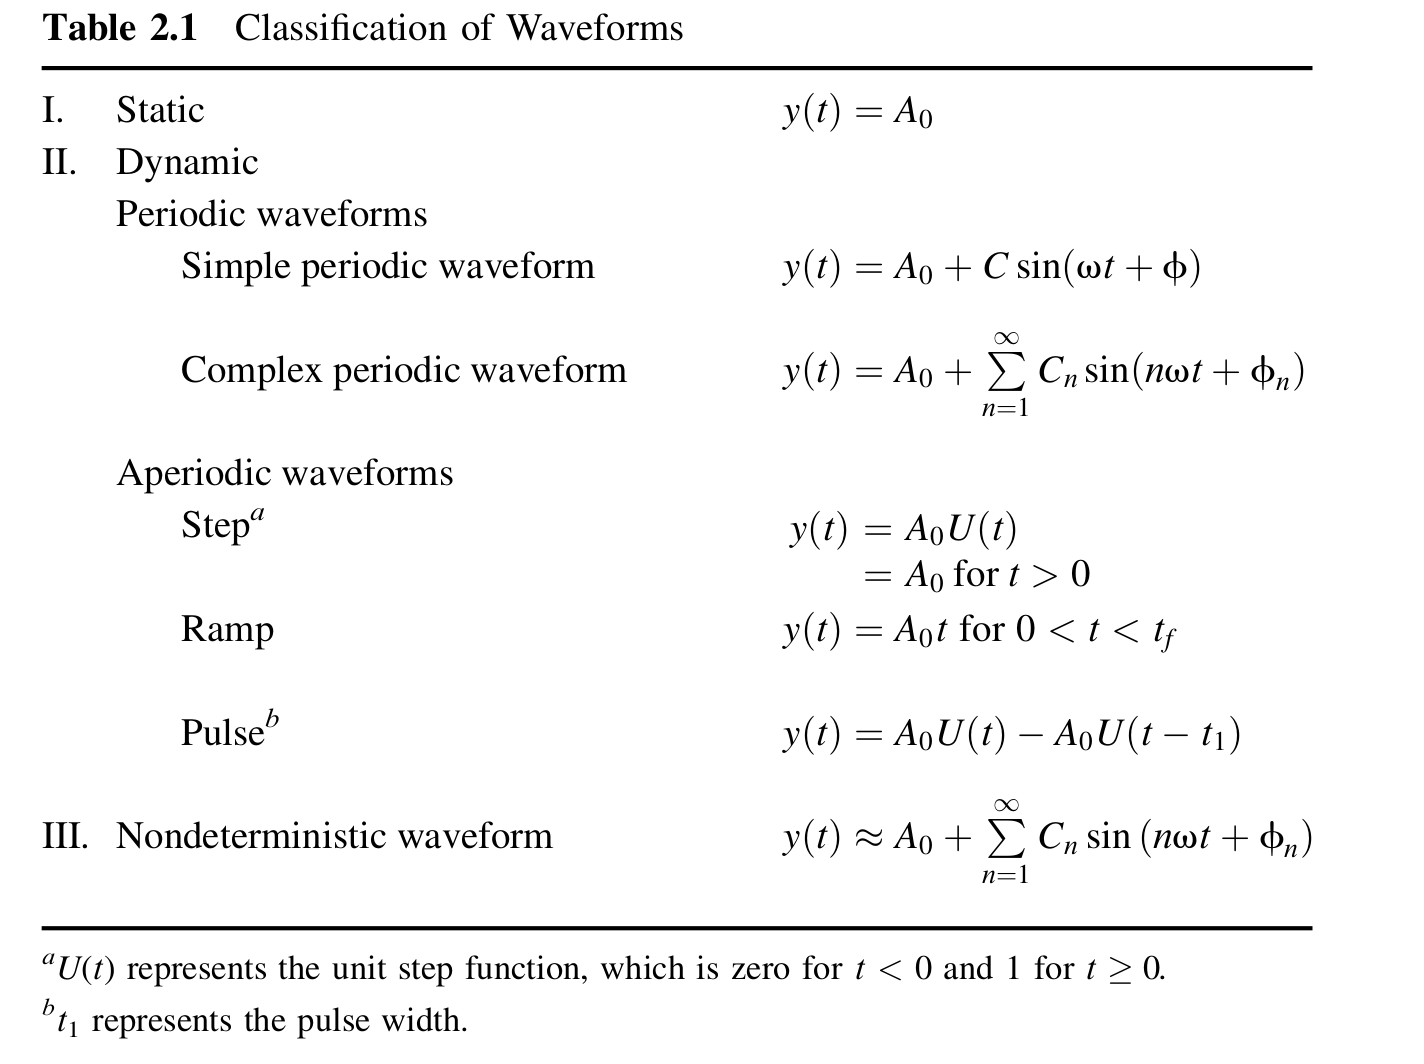
\includegraphics[scale=.15]{table_2_1.png}

\btVFill
\tiny{Table 2.1 : Theory and Design for Mechanical Measurements}	
\end{frame}

\end{document}
